\section{Velvet Interlinks}\label{sec:velvet}
More recently, velvet forks have been introduced~\cite{velvet}. In a
velvet fork, blocks created by upgraded miners (called \emph{velvet blocks}) are
accepted by unupgraded miners as in a soft fork. Additionally, blocks created by
unupgraded miners are also accepted by upgraded miners. This allows the protocol
to upgrade even if only a minority of miners chooses to upgrade. To maintain
backwards compatibility and to avoid causing forks, the additional data included
in a block is \emph{advisory} and must be accepted whether it exists or not.
Even if the additional data is invalid or malicious, upgraded nodes (in this
context also called \emph{velvet nodes}) are forced to accept the blocks. The
simplest approach to velvet fork the chain for interlinking purposes is to have
upgraded miners include the interlink pointer in the blocks they produce, but
accept blocks with missing or incorrect interlinks. As we show in the next
section, this approach is flawed and susceptible to unexpected attacks. A
surgical change in the way velvet blocks are produced is necessary to achieve
proper security.

In a velvet fork, only a minority of honest parties needs to support the protocol
changes. We refer to this percentage as the ``velvet parameter''.

\begin{definition}[Velvet Parameter]
	The \emph{velvet parameter} $g$ is defined as the percentage of honest parties
	that have upgraded to the new protocol. The absolute number of honest upgraded
	parties is denoted $n_h$ and it holds that
	$n_h = g (n - t)$.
	\label{defn:velvet_honest_majority}
\end{definition}

Velvet forks maintain backwards and forwards compatibility. This requires any block produced by upgraded miners to be accepted by unupgraded nodes (as in a soft fork), but also blocks produced by unupgraded miners to be accepted by upgraded nodes. For the particular case of superblock NIPoPoWs under velvet forks, upgraded miners must include the interlink data structure within their blocks, but must also accept blocks missing the interlink structure or containing an invalid interlink. Unupgraded honest nodes will produce blocks that contain no interlink, while upgraded honest nodes will produce blocks that contain truthful interlinks. Therefore, any block with invalid interlinks will be adversarially generated. However, such blocks cannot be rejected by the upgraded nodes, as that would give the adversary an opportunity to cause a hard fork.

A block generated by the adversary can thus contain arbitrary data in the interlink and yet be adopted by an honest party. Because the honest prover is an upgraded full node, it can determine what the correct interlink pointers are by examining the whole previous chain, and can thus deduce whether a block contains invalid interlink data. In that case, the prover can simply treat such blocks as unupgraded. In the context of the attack that will be presented in the following section, we examine the case where the adversary includes false interlink pointers.

A correct interlink pointer of a block $b$ for a specific level $\mu$ is a pointer to the most recent among all the anecestors of $b$ that have achieved at least level $\mu$. We will refer to correct interlink pointers as \emph{smooth pointers}. Pointers of the 0-level \textit{(previds)} are always smooth because they are also validated by the unupgraded protocol before adoption. Thus the previd of an
honestly adopted block cannot be invalid.

\begin{definition}[Smooth Pointer]
  A \emph{smooth pointer} of a block $b$ for a specific level $\mu$ is the interlink pointer to the most recent $\mu$-level ancestor of $b$.
	\label{defn:smooth_pointer}
\end{definition}

A non-smooth pointer may not point to the most recent ancestor of level $\mu$ or even point to a superblock of a fork chain, as shown in Figure~\ref{fig:false_interlink}.

\begin{figure}[h]
	\begin{center}
		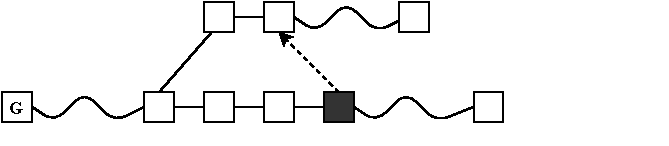
\includegraphics[width=0.9\columnwidth]{figures/false_interlink.pdf}
	\end{center}
    \caption{A non-smooth pointer of an adversarial block, colored black, in an honest party's chain.}
	\label{fig:false_interlink}
\end{figure}

In the same manner it is possible that a false interlink contains arbitrary pointers to blocks of any chain as illustrated in Figure~\ref{fig:thorny_block}. The interlink pointing to arbitrary directions resembles a thorny bush, so we will refer to blocks containing false interlink information as \emph{thorny}.

\begin{definition}[Thorny Block]
	A \emph{thorny block} is a block that contains at least one non-smooth interlink pointer.
	\label{defn:thorny_block}
\end{definition}

\begin{figure}[h]
	\begin{center}
		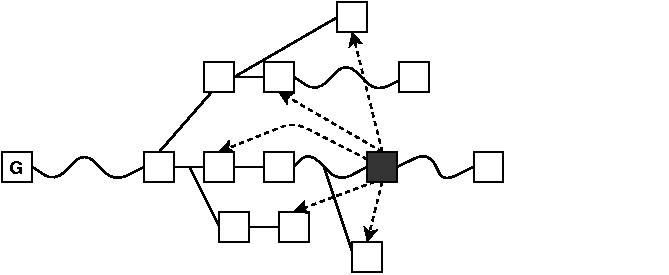
\includegraphics[width=0.9\columnwidth]{figures/thorny_block.pdf}
	\end{center}
	\caption{A thorny block appended to an honest party's chain.
	The dashed arrows are interlink pointers.}
	\label{fig:thorny_block}
\end{figure}

Contrary to thorny blocks, \emph{smooth} blocks are blocks containing no interlink structure or containing only smooth pointers in their interlink. All blocks produced by honest parties are smooth, as unupgraded honest miners produce blocks with no interlink and upgraded honest miners produce interlinks containing only smooth pointers.

\begin{definition}[Smooth Block]
	A \emph{smooth block} is any block that is not thorny.
	\label{defn:smooth_block}
\end{definition}
